% ==================================================================
\section{Municipal soy accounting}\label{app:accounting}
% ==================================================================
% Pipeline step 00 (00_data_preparation) and step 01.

Throughout the appendices, $m$ and $n$ index Brazil's 5{,}570
municipalities, $p\in\{\text{bean},\text{oil},\text{cake}\}$ the three soy
products, and $i,j$ countries; matrices and vectors are set in bold.
One operation recurs throughout the subnational reconstruction:
a national total is distributed across municipalities in proportion to
an observable weight, as listed in Table~\ref{tab:weights} of the
Methods document. The released pipeline checks each such allocation
against its national total at run time and halts on any violation.

\subsection{Data assembly and domestic-use estimation}\label{subsubsec:domuse}
\label{subsubsec:assemble}
Five rules complete the allocation weights of Table~\ref{tab:weights}
and the assembly of the municipal accounts:
\begin{enumerate}
\item exports declared without a municipality of origin are
redistributed across the declared exporters of the same product and
destination in proportion to their volumes, thus conserving national
totals (undeclared imports are negligible);
\item the crushing-capacity weight is constructed by dividing each
state's reported capacity total equally among its active plants, as
per-plant capacities are not published; the cost of this assumption is
quantified in the Technical validation
(Section~\ref{subsec:val-inputs});
\item the biodiesel-capacity weight attributes each plant's capacity
to soy in proportion to its macro-region's soy feedstock share;
\item municipal oil and cake output follow from the allocated crush:
each year's oil and cake yields are the ratios of the national oil and
cake production to the crushed bean quantity in the FAO balance of
that year, giving approximately 20\% oil and 75\% cake with a 5\%
processing loss, in line with the yields reported in the literature
\cite{smaling2008soy,dei2011soybean};
\item all geometries are projected to SIRGAS~2000 / Brazil Polyconic
(EPSG:5880); each municipality is represented by its administrative
centre, and the straight-line distances between these centres provide
the transport costs of Appendix~\ref{app:transport}.
\end{enumerate}
The treatment of stock changes, summarized in the last row of
Table~\ref{tab:weights}, is derived in Appendix~\ref{app:balancing}.

% ==================================================================
\section{Livestock systems and feed demand}\label{app:livestock}
% ==================================================================
% Pipeline steps 02-03.

\subsection{Production-system disaggregation}
IBGE municipal herd counts are divided into extensive and intensive
chickens; extensive, intensive and industrial pigs; and grassland- and
mixed-based cattle and buffalo, each split into dairy and meat. The
municipal share of each system is the area-weighted zonal sum of the
2010 FAO gridded livestock rasters (GLW3) and the GLEAM ruminant
production-system map, normalized across the systems of each species;
where a municipality reports a herd in the run year but had no gridded
animals in 2010, the state-mean share is substituted. Pigs follow the
raster shares directly. For poultry, the extensive share of the total
flock forms backyard birds, and the intensive share splits into layers
(the reported laying hens) and broilers (the rest; all birds where
layers are unreported). Feedlot cattle, reported only in the
agricultural census, are the 2006 census counts scaled by the national
confinement growth factor of the run year (e.g.\
$4.38/3.46\approx1.27$ for 2013, from ABIEC/Athenagro), holding the
municipal pattern fixed; the remaining cattle are split into grassland
and mixed systems by the raster shares, with dairy identified by
milked cows and meat as the residual. Buffalo use the municipal
milked-cow ratio of cattle as the dairy proxy. Each species'
subsystems partition its reported herd exactly.

\subsection{Feed demand and national rescaling}
Each herd is multiplied by its GLEAM per-animal intake (annual dry-matter
intake times the share sourced from soybeans and soy cake, converted to
as-fed tonnes at 88\% dry matter). One national factor per product then
rescales the bottom-up totals to the FAO national feed figures,
preserving the spatial and cross-system distribution.
Municipal feed demand for beans and cake is the sum over systems. Holding
the 2010 system shares fixed over the study period is a simplification:
herd sizes remain annual, misclassification affects only how a herd is
split across intake intensities, and the national rescaling bounds the
aggregate error, which grows with distance from the 2010 reference year.

% ==================================================================
\section{National balancing and trade reconciliation}\label{app:balancing}
% ==================================================================
% Pipeline steps 04-05.
For each product, the national commodity balance imposes the supply--use
identity: production, imports and stock withdrawals (supply) equal
exports, food, feed, seed, processing and other uses (use). The trade
harmonisation collapses destinations absent from the FABIO/FAOSTAT
bilateral list into a rest-of-world aggregate; it aligns
classifications only and applies no rescaling. The balance items are
rescaled proportionally, with each item's municipal distribution as
weight, after the national residual has been moved into the stock
term. A net national stock withdrawal is carried on the supply side:
the drawdown is distributed across municipalities by the stock weights
(storage capacity for beans, production for oil and cake) and added to
municipal supply. A drawdown is a genuine source of current-year
supply, and this treatment alone keeps every municipal use
non-negative, as required by the re-export inversion of
Appendix~\ref{app:tracing}. Net additions remain on the use side. As
each year is solved independently, tonnes supplied from a drawdown,
physically grown in earlier years, inherit the current year's soy-area
intensity (Appendix~\ref{app:footprint}). Finally, each municipality's
product balance defines its surplus,
$\max(\text{supply}^p_m-\text{use}^p_m,0)$, and deficit,
$\max(\text{use}^p_m-\text{supply}^p_m,0)$, which drive the
inter-municipal flows of Appendix~\ref{app:transport}; the two totals
match by construction after the rescaling, as required by the balanced
transportation problem. The national residual itself cannot be
resolved into flows; it is retained as FABIO's signed balancing column
and re-enters the model as a dedicated final-demand category
(Appendices~\ref{app:nesting} and \ref{app:footprint}).

% ==================================================================
\section{Optimal-transport formulation}\label{app:transport}
% ==================================================================
% Pipeline step 07 (07_transport_R.R) for the Euclidean model; step 06
% (06_transport_cost.R) + transport_lp/ (Pyomo+HiGHS port of Stefan's GAMS
% model) for the multimodal variant. Multimode solved 2010-2022 (2021
% infeasible), central cost parameters, water cargo proxied before 2017;
% see docs/multimode_transport_results.md.

\subsection{The Euclidean model}\label{subsubsec:euclid}
For each product
$p$, the inter-municipal flow matrix $\mathbf{F}^p$ solves the balanced
transportation problem
\begin{equation}\label{eq:ot}
  \mathbf{F}^{p}=\argmin_{\mathbf{F}\ge0}\ \sum_{m,n}F_{mn}\,d_{mn}
  \quad\text{s.t.}\quad
  \sum_{n}F_{mn}=\text{surplus}^p_m,\ \
  \sum_{m}F_{mn}=\text{deficit}^p_n,
\end{equation}
where $d_{mn}$ is the straight-line distance between the administrative
centres of municipalities $m$ and $n$ (Appendix~\ref{app:accounting}) (the two margins are balanced beforehand by
proportionally scaling the larger one). The problem is solved exactly by
the network-simplex algorithm (R package \texttt{transport}
\cite{schuhmacher2023transport}), separately for beans, oil and cake.

\subsection{The multimodal network variant}\label{subsubsec:multimode}
To test whether the straight-line metric distorts the allocation, the
same municipal surpluses and deficits are re-solved on a multimodal
representation of Brazil's logistics network, generalizing the
single-year (2013) intermodal model of Trsek \cite{trsek2022} to the
years 2010--2022. The variant has three building blocks:
\begin{enumerate}
\item the network: roads (OpenStreetMap, simplified to a 5\,km grid),
railways (ANTT lines and stations) and waterways (DNIT rivers with
ANTAQ ports). A tonne may travel by road directly, or by road to a
rail or waterway terminal, along that network, and onwards by road to
its destination;
\item the costs: every leg is priced at a unit cost per tonne-km that
depends on the mode (road 0.013--0.174, rail 0.006--0.065, water
0.004--0.032~USD), and changing modes carries a switching charge
(0.74--2.57~USD per tonne); the central runs use the midpoints of
these ranges, taken from the freight-cost literature compiled in
\cite{trsek2022};
\item the capacities: a rail or waterway corridor cannot carry more of
a product than it was observed to carry, from ANTT
origin--destination rail records (all study years) and ANTAQ port
statistics (observed from 2017 onwards; earlier years are proxied with
the 2017 records, as ANTAQ's pre-2017 archives are currently
unavailable).
\end{enumerate}
The resulting minimum-cost flow problem is solved with the open-source
HiGHS solver; the 2021 problem is infeasible on the current inputs and
is excluded from the comparison.

% ==================================================================
\section{Origin tracing and re-export disentangling}\label{app:tracing}
% ==================================================================
% Pipeline steps 08 and 12.

\subsection{Linking origin municipalities to importing countries}\label{subsubsec:exportlink}
The transport flows of Appendix~\ref{app:transport} record only what
moves between municipalities, so the part of each municipality's supply
that stays and is used at home is added on the diagonal,
\begin{equation}\label{eq:augment}
  \tilde F^p_{mn} \;=\; F^p_{mn} \;+\;
  \mathbf{1}[m=n]\,\big(\text{supply}^p_m-\text{surplus}^p_m\big),
\end{equation}
so that the rows of $\tilde{\mathbf{F}}^p$ sum to total municipal supply
and its columns to total municipal use. Every exported tonne is then
unwound to its origin (Figure~\ref{fig:tracing}),
\begin{equation}\label{eq:src2exp}
  X^p_{mj}=\delta^p_m\sum_{n}\phi^p_{mn}\,E^p_{nj},
\end{equation}
where $E^p_{nj}$ are the observed exports of municipality $n$ to country
$j$; the sourcing share
$\phi^p_{mn}=\tilde F^p_{mn}/\sum_{m'}\tilde F^p_{m'n}$ is the fraction
of $n$'s total use that originated in municipality $m$ (including $m=n$);
and the domestic-origin share
$\delta^p_m=(\text{supply}^p_m-\text{imports}^p_m)/\text{supply}^p_m$
strips out quantities of foreign origin (withdrawal-supplied tonnes count as
domestic under the supply-side stock treatment;
Appendix~\ref{app:balancing}).
Local consumption is traced with the same formula through a synthetic
domestic column added to the export table (for beans net of the crush, which
is traced through the oil and cake chains instead), and oil and cake are
traced one step further back, to the bean-growing municipalities, by
premultiplying their origin-to-destination matrices with the bean sourcing
shares and the bean domestic-origin share.

\subsection{Re-export disentangling}\label{subsubsec:reexport}
To attribute internationally traded soy to its true origin, bilateral
trade is disentangled with the standard Leontief-type inversion of
physical trade-linkage accounting \cite{kastner2011tracing}: trade is
normalized by destination use, the infinite re-export chain is summed
by matrix inversion, and retaining the domestically produced
quantities yields the origin-to-consumption matrix,
\begin{equation}\label{eq:reex}
  \mathbf{R}=\mathbf{T}\,\hat{\mathbf{u}}^{-1},
  \qquad
  (\mathbf{I}-\mathbf{R})^{-1}=\sum_{k=0}^{\infty}\mathbf{R}^{k},
\end{equation}
where $\mathbf{T}$ is the bilateral trade matrix, $\hat{\mathbf{u}}$
the diagonalized vector of total use by region, $R_{ij}$ the share of
region $j$'s use supplied by imports from region $i$, and
$\mathbf{R}^{k}$ carries the flows re-exported $k$ times, so the
inverse sums chains of every length. The departure from
the published method is the regional dimension: for the soy products
Brazil is replaced by its 5{,}570 municipalities, enforced throughout
the processing of the trade data so that no national Brazilian record
re-enters the inversion. The inversion treats the soy available in a
region as one well-mixed pool: local production and incoming shipments
blend in proportion to their volumes, and every user of the pool
receives the same origin mix, as is natural for a bulk commodity
blended in silos. Which municipality exports to which country is
observed in the customs data, so the assumption does not touch that
step; it fills in only where an exporting municipality's soy came from
within its catchment, and how soy is passed on when a country
re-exports it. What it cannot represent is a buyer who deliberately
selects soy of a specific origin, as European importers do under the
Amazon Soy Moratorium: such origin-specific contracting is not
resolved. The inversion is computed exactly by a sparse solver,
with a dense fallback and, as a last resort, a small diagonal ridge to
lift a genuine unit eigenvalue (a commodity whose recorded global
trade is entirely re-exported); the years requiring the ridge are
documented with the released code.

% ==================================================================
\section{FABIO backends and temporal coverage}\label{app:nesting}
% ==================================================================
% Pipeline steps 13-19.

The FABIO v2 build exists only from 2010 onwards; for 2001--2009 the
pipeline switches to four inputs from the FABIO v1.1 build: the full
bilateral trade detail, the land-use extension, the feedstock
optimisation results, and the v1 balance sheets (the v2 balance file
contains only placeholder rows before 2010). Version bridges map
through stable FAO item codes, and the v1.1 land-use extension, which
reports total agricultural land rather than v2's cropland, is
converted to the per-process intensity vector through the same
mapping; soy is cropland under both definitions, so the soy land
footprint is unaffected, but non-soy land intensities are not
comparable across vintages. The seam is quantified on the overlap
years 2010--2013, run through both chains end to end: in the two clean
overlap years totals differ by $-6\%$ (2011) and $-8\%$ (2013, v1.1
low) with cross-country correlations of consumer footprints of 0.988
and 0.992 (the 2012 v1.1 build halts at the re-export conservation
check, and 2010 diverges through a disagreement between the
balance-sheet vintages), so pre-2010 levels are reported unadjusted.
One usage caveat: Brazil's domestic footprint is about a third
lower on v1.1, so cross-vintage statements about Brazil-domestic use
are restricted to 2010 onwards.

% ==================================================================
\section{Land-use footprint accounting}\label{app:footprint}
% ==================================================================
% Pipeline steps 20-21.

\subsection{Footprint calculation}\label{subsubsec:stressor}
With $e_i=\text{land}_i/x_i$ the land intensity of process $i$ (its
direct soy area per unit of output; Section~\ref{subsec:footprint}), the
footprint is the standard intensity--Leontief--demand product
\begin{equation}\label{eq:fp}
  \mathbf{H}=\hat{\mathbf{e}}\,\mathbf{L}\,\mathbf{Y},
\end{equation}
where $\hat{\mathbf{e}}$ is the diagonal matrix of the land intensities,
$\mathbf{L}$ the Leontief inverse of the nested system, $\mathbf{Y}$ final
demand aggregated to consumer countries, and $H_{ij}$ the hectares of soy
land in origin municipality $i$ embodied in country $j$'s consumption.
Stock additions and the balancing category are removed from final demand
before aggregation: stock drawn down in year $t$ embodies land use of
earlier years, and retaining it as negative year-$t$ demand would
attribute negative footprints to producer regions in drawdown years;
EXIOBASE inventory changes are treated analogously. The
food system and the non-food background traced through EXIOBASE
\cite{stadler2018exiobase} contribute additively to each
consumer's total. Footprints by consumed product are obtained by
restricting $\mathbf{Y}$ to selected commodity groups (e.g.\ dairy, meat)
before applying \eqref{eq:fp}.

\subsection{Origin attribution and grid refinement}\label{subsubsec:attribution}
The biome assignment intersects each municipality's interior point with
the biome layer; points falling outside every biome polygon are assigned
the nearest biome. A destination's frontier share is the fraction of its
origin footprint located in frontier municipalities, with the frontier as
defined in Section~\ref{subsec:footprint}. For visualization, per-municipality embodied production can
optionally be distributed onto 30\,m MapBiomas soy pixels, each pixel of a
municipality carrying that municipality's per-pixel share for the given
consumer country; this refinement is illustrative and does not affect the
reported results.

% ==================================================================
\section{Validation and uncertainty analysis}\label{app:validation}
% ==================================================================
% Pipeline steps 10-11 (10_create_benchmarks.R, 11_analyse_benchmarks.R)
% + code/analysis/{sens_inputs.sh,fig_dest_sets.py}. Companion to the
% Technical validation working document.

\subsection{Benchmark and baseline}\label{subsubsec:benchmarks}
The comparison sample is built from the origin-to-importer flows
$X^p_{mj}$ of Appendix~\ref{app:tracing}, the Trase composite, and the
downscaling baseline, defined as national exports to each destination
allocated to municipalities in proportion to their share of
domestic-origin soybean supply: every importer draws from the same
municipal map, importers differ only in total volume, and the baseline
contains no supply-chain structure by construction. All three sources
are converted to bean equivalents with the national crush ratio and
summed over beans, oil and cake. Trase flows with unknown origin
municipality are excluded, destinations are harmonized to the
bilateral-trade classification, and the sample comprises all
soy-producing municipalities crossed with the destinations recording
positive exports in both benchmark and model. Brazil, which enters the
tables as the destination of domestic use, is excluded wherever
importers are compared or weighted.

\subsection{Agreement by importer}\label{subsubsec:byimporter}\label{sec:val-annex}
Figures~\ref{fig:top70} and~\ref{fig:bottom5} unpack the
volume-weighted average reported in the Technical validation section
at the two ends of the volume distribution: the four importers that
together take 70\% of the Trase-recorded 2010--2022 volume (China, the
Netherlands, Thailand and Spain), and the five smallest importers with
matched flows in every year (Cuba, Israel, the United Arab Emirates,
Greece and Australia, 0.1--1.5\,Mt each over the whole period). Each
figure shows the mean correlation over its importer set and, below it,
the full per-importer scores per year for the three allocation
variants.

\begin{figure}[H]
\centering
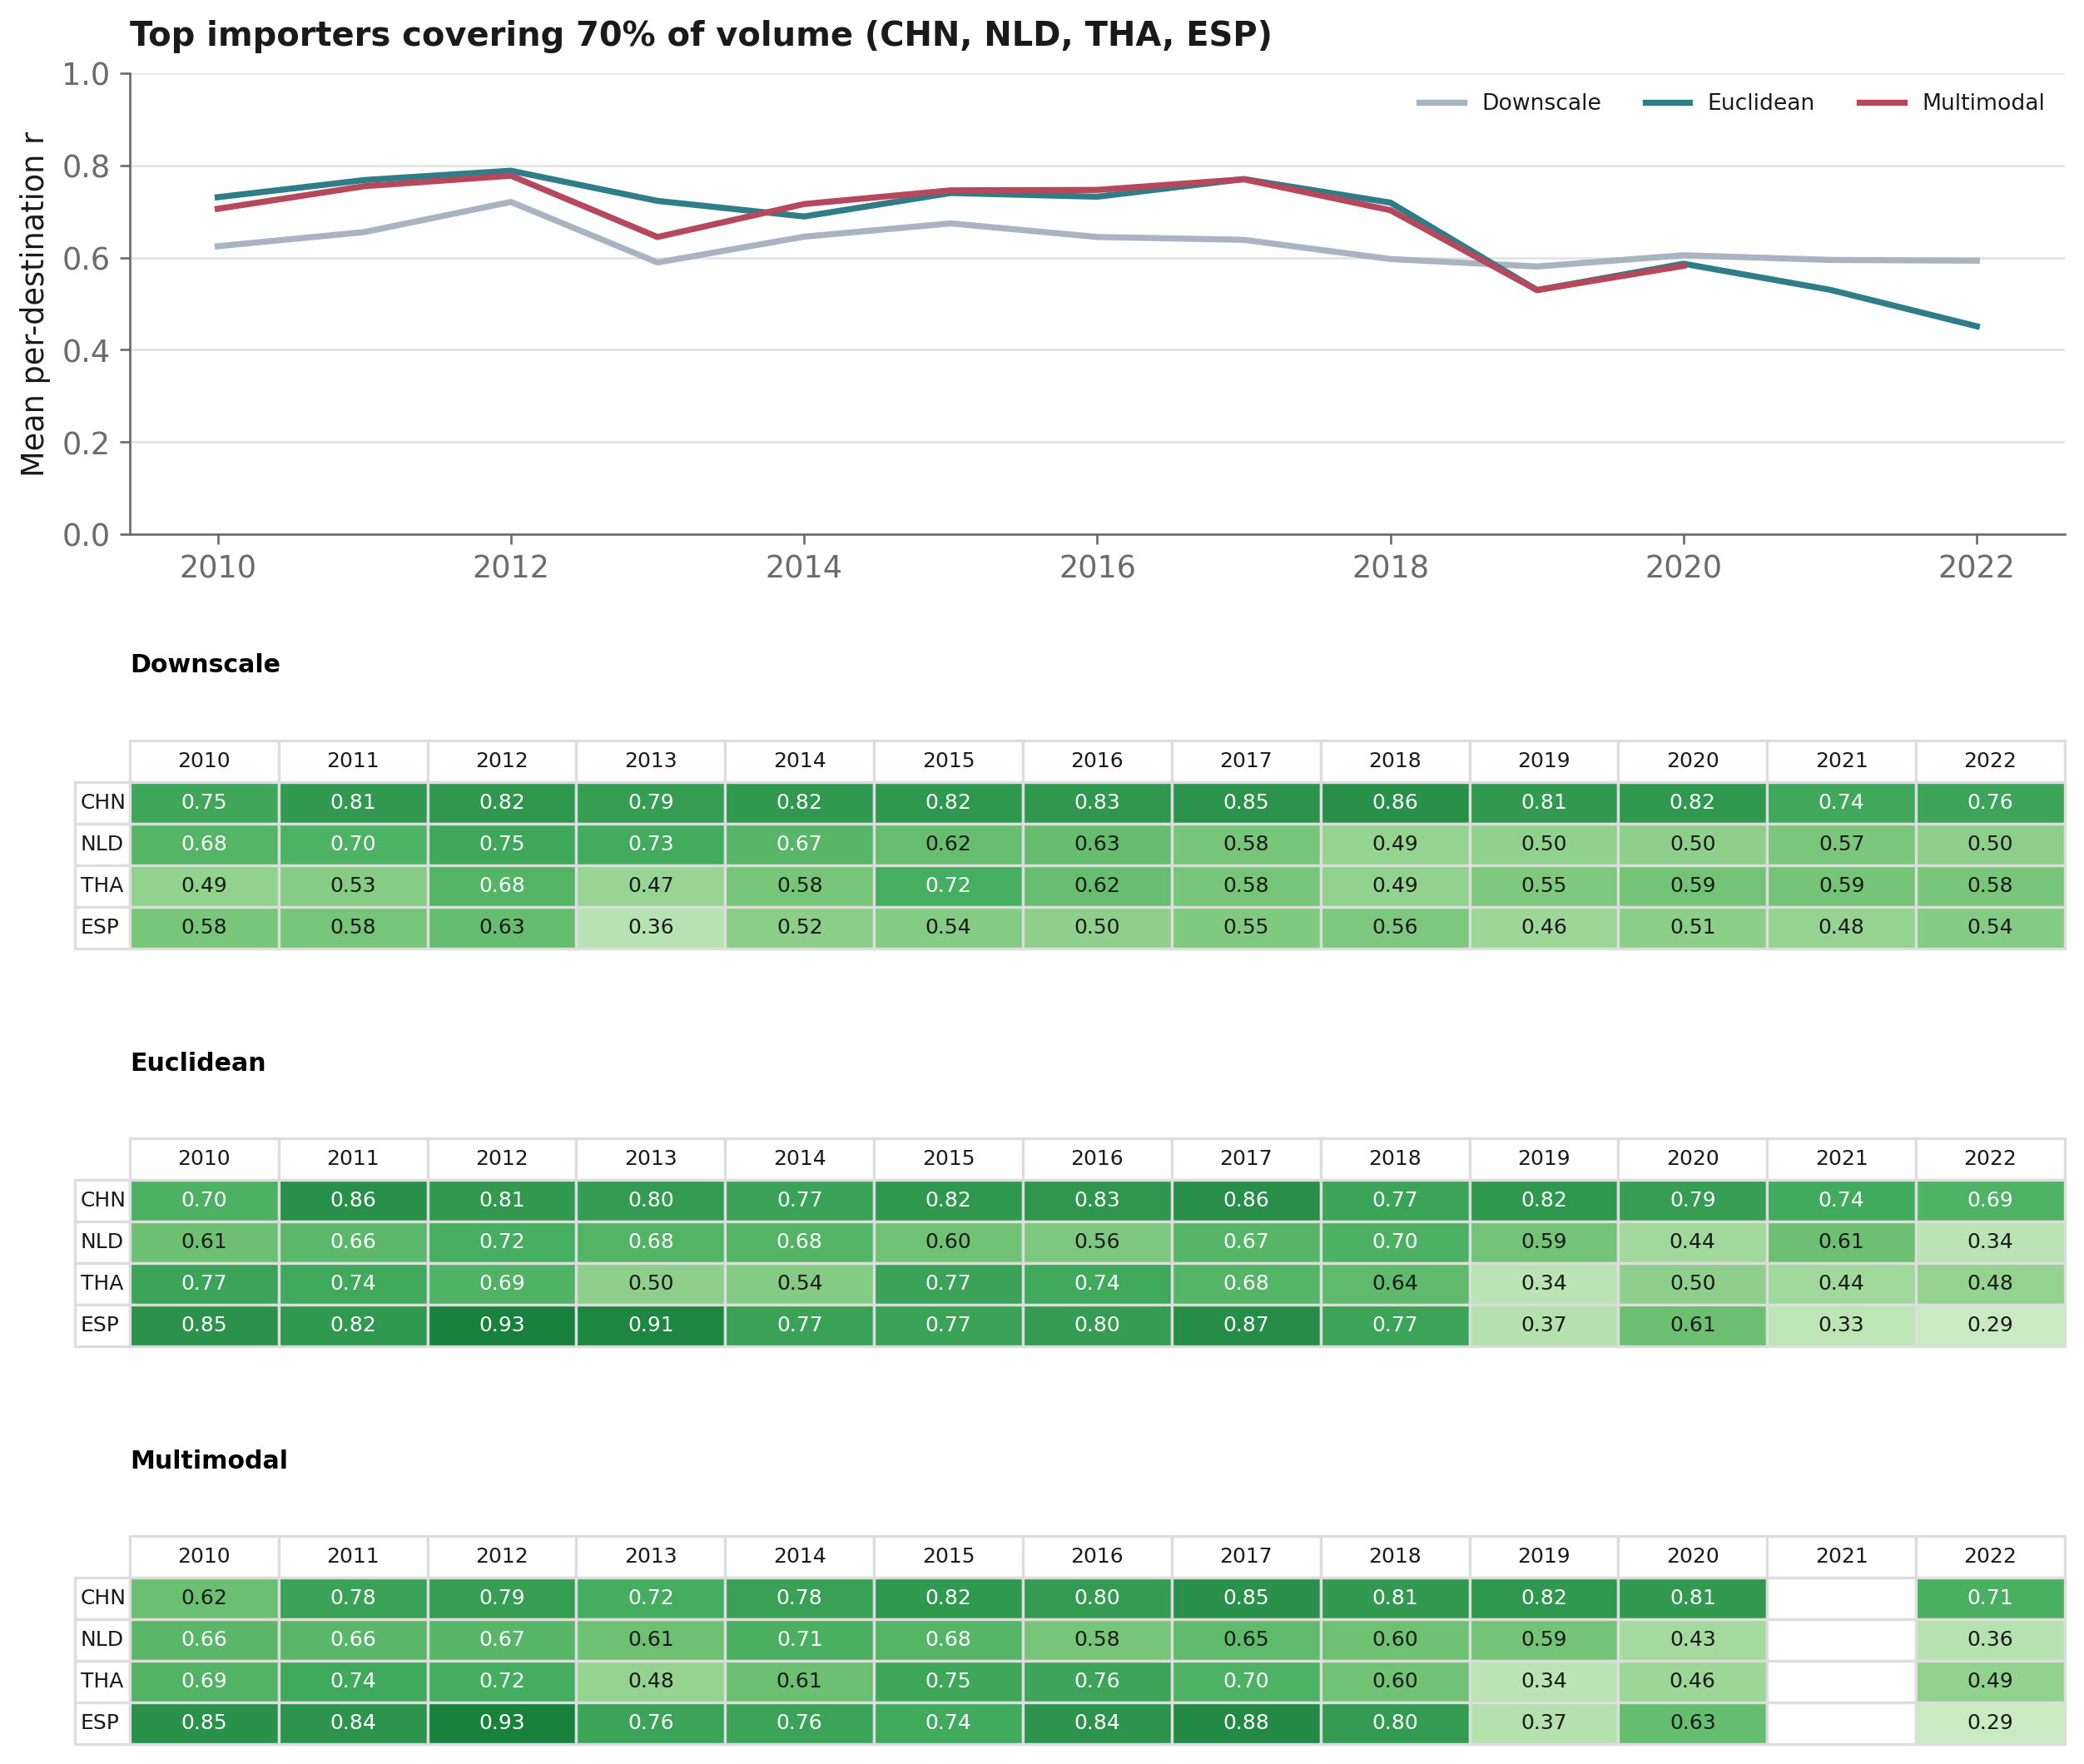
\includegraphics[width=\textwidth]{figures/fig_dest_top70.png}
\caption{Per-destination correlation with Trase for the four importers
covering 70\% of the 2010--2022 volume. The line plot shows the mean
over the four importers; the tables give the per-importer scores per
year for each allocation variant (colour scale from 0, white, to 1,
dark green; the multimodal variant has no 2021
solve).}\label{fig:top70}
\end{figure}

\begin{figure}[H]
\centering
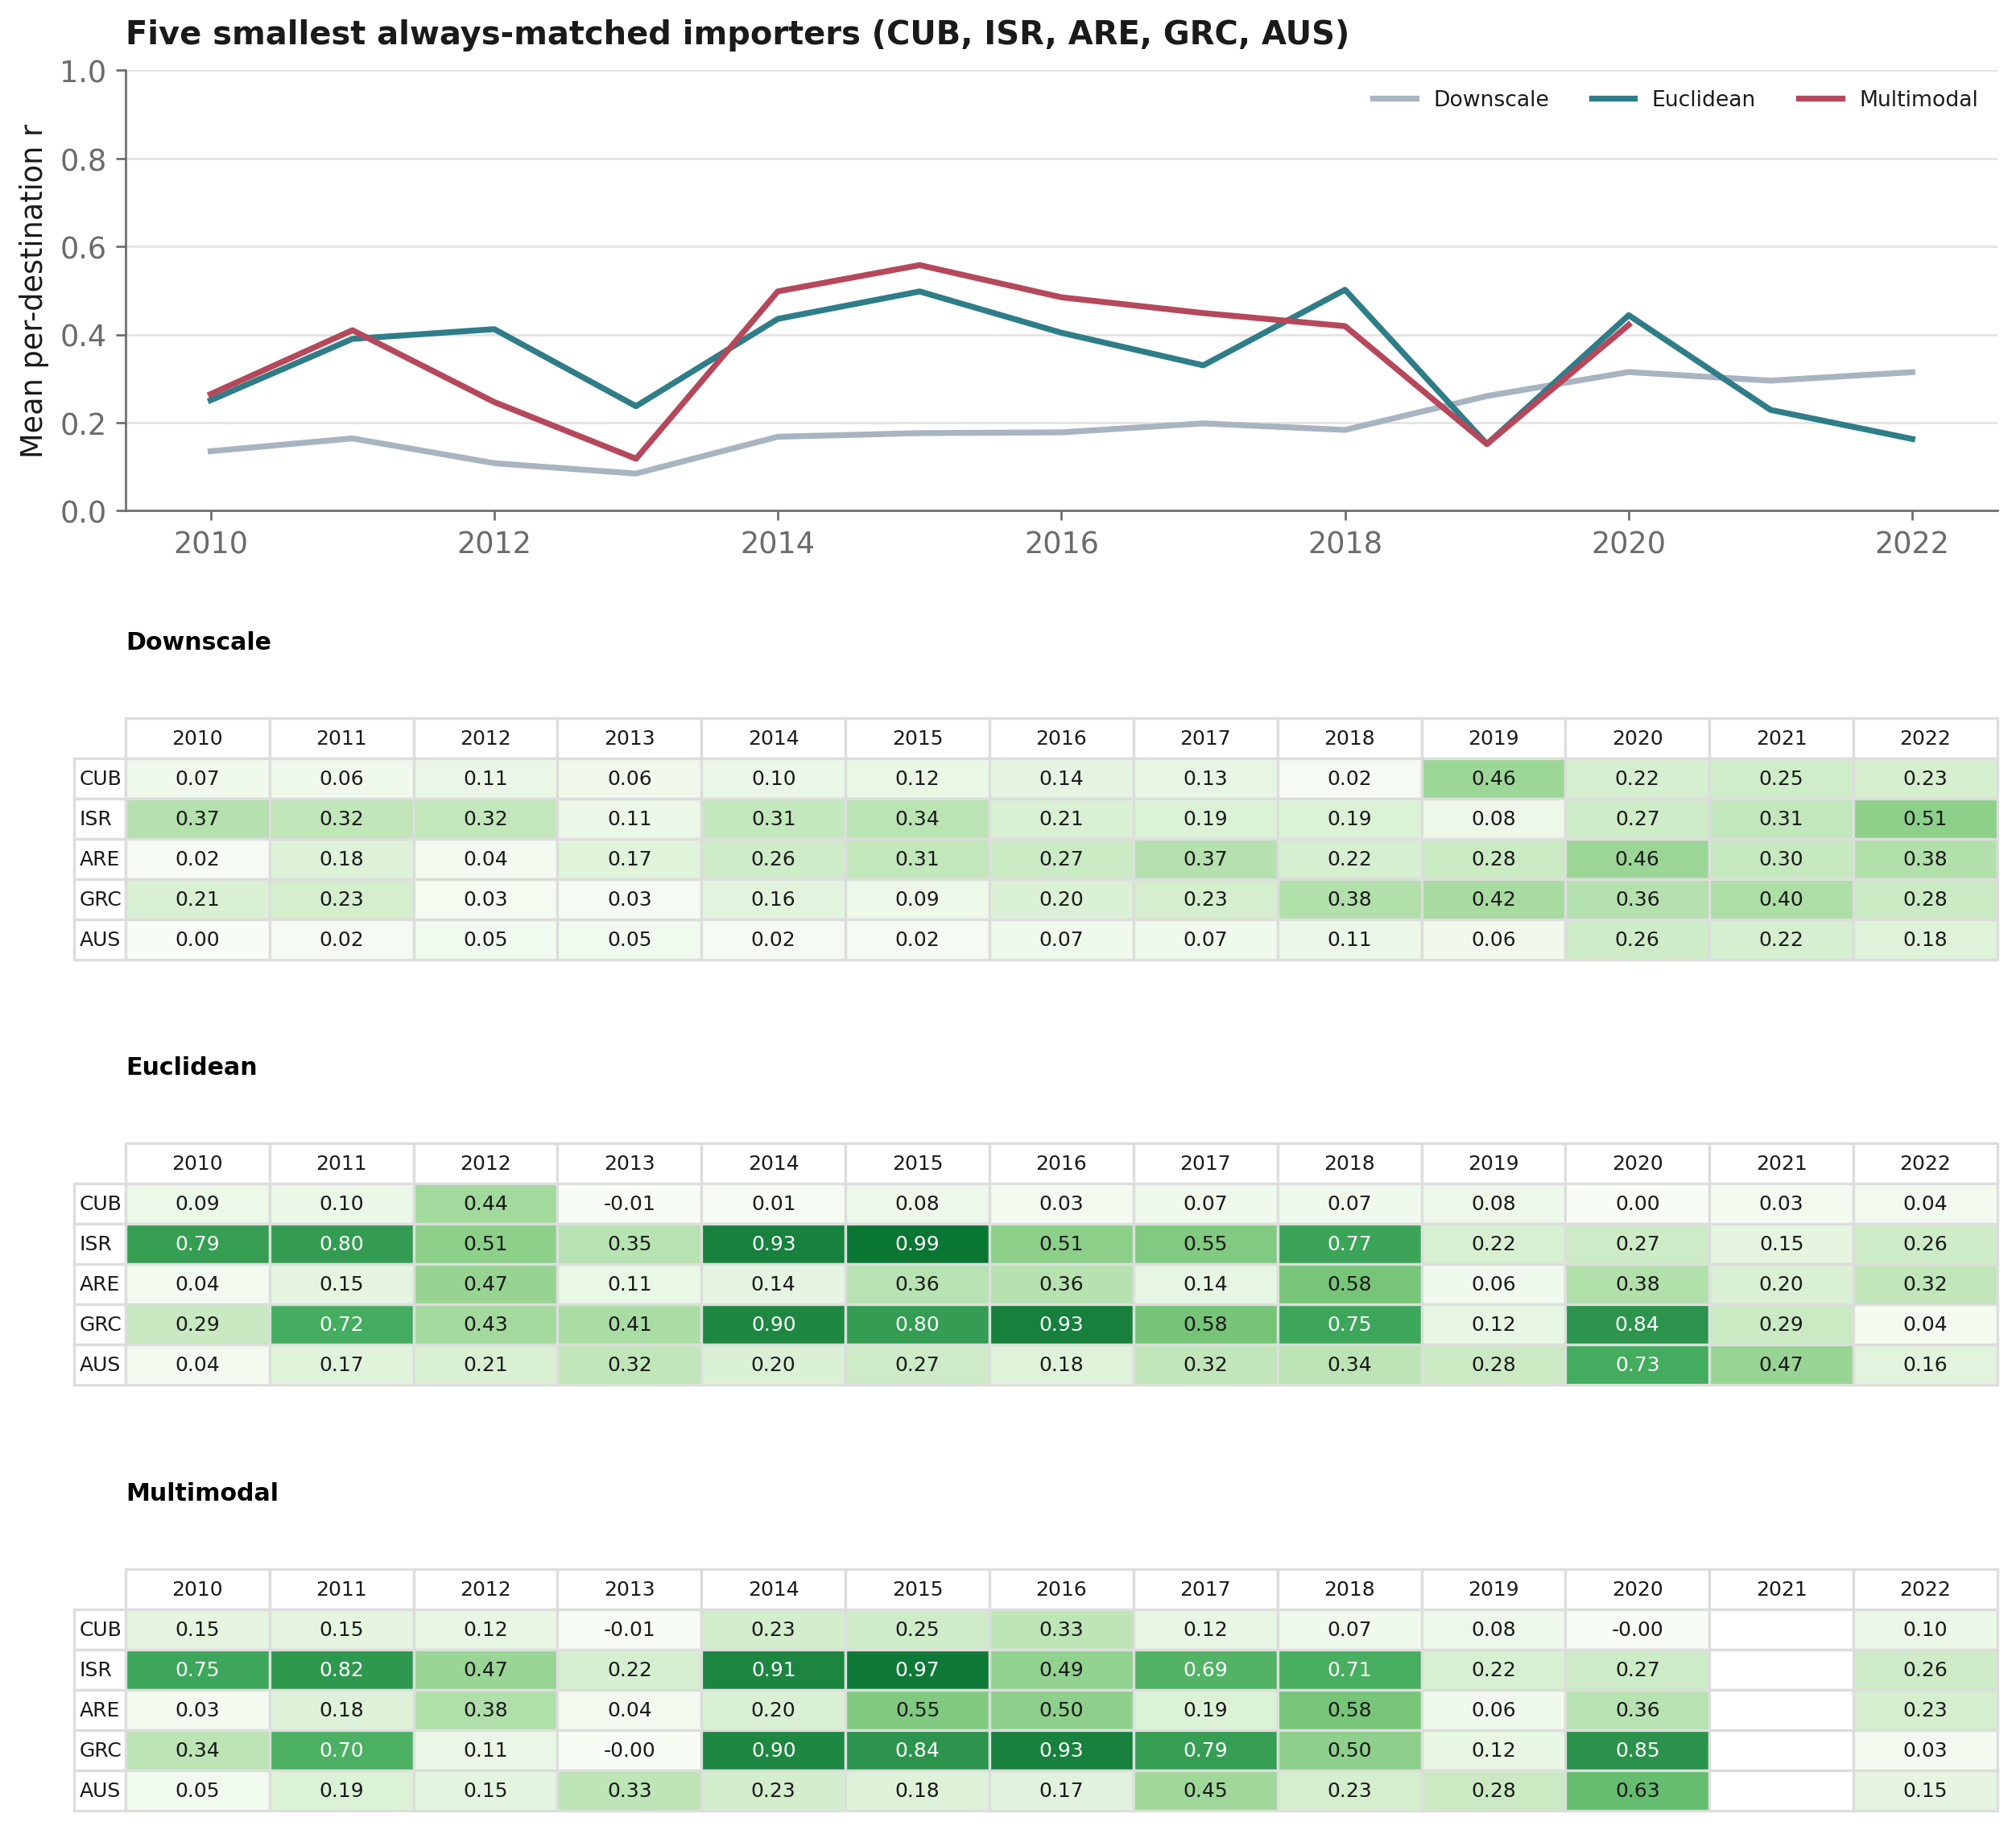
\includegraphics[width=\textwidth]{figures/fig_dest_bottom5.png}
\caption{As Figure~\ref{fig:top70}, for the five smallest importers
matched in every year. At this volume level, three orders of magnitude
below China, the correlations scatter from slightly negative to above
0.9 with no persistence from year to year: individual small-importer
results carry little information.}\label{fig:bottom5}
\end{figure}

\subsection{Perturbation recipes of the input-sensitivity screen}\label{subsubsec:perturb}
Crush location. Each state's fixed capacity total is redistributed
over its plant municipalities in proportion to a weight $k_m$:
one in the baseline (equal split), municipal soybean production in the
production-proportional variant, and $k_m \sim \mathrm{Exp}(1)$ drawn
independently per plant in the random variants, which makes every
split of the state total equally likely (a uniform Dirichlet
distribution over the shares); ten seeds give ten capacity maps. The
allocation-sharpness variants leave the split untouched and raise the
allocation weight to $\mathrm{cap}_m^{\gamma}$ with
$\gamma \in \{0.5, 2\}$.

Feed rates. The per-head bean and cake rates of every livestock system
are multiplied by independent mean-one lognormal factors,
\begin{equation}\label{eq:feedjitter}
  f \;=\; \exp\!\big(\mathcal{N}(-\sigma^2/2,\ \sigma^2)\big),
  \qquad \sigma = 0.3 ,
\end{equation}
drawn separately for the bean and the cake rate of each system; ten
seeds give ten parametrisations. Because national feed totals are
rescaled to the FAO commodity balance after the multiplication
(Appendix~\ref{app:livestock}), a factor common to all systems cancels
exactly, and only the relative system mix moves the spatial
allocation. The herd-composition variant replaces the 2010-frozen
municipal system shares with state averages.
